\chapter{Disegnare} \label{cap:disegnare}

\section{Comandi di movimento – Disegno - Uso delle variabili}

\subsection{I comandi fondamentali} \label{sec:comandi-fondamentali}

Il programma consente di creare grafica mediante il movimento di una  "tartaruga " che obbedisce a precisi comandi. Vediamo subito un esempio.

Apri un nuovo documento di testo e scrivi questo comando:

\vskip 1cm

\begin{scriptsize}
\begin{minipage}{01.0\textwidth}
\begin{itemize}[itemsep=-3pt,parsep=2pt]
\item[] \hspace{0.5cm} \textbf{HOME} 
\end{itemize}
\end{minipage}
\end{scriptsize}

\vskip 1cm

Vedrai che è apparsa la tartaruga in mezzo al foglio con la testa verso l'alto:

\begin{figure}[H]
   \centering
   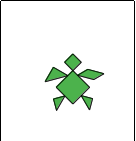
\includegraphics[width=3.0cm,trim=4 4 8 4,clip]{./images/disegnare/disegnare-1.png}
   \label{dis-1}
\end{figure}

Ora aggiungi un altro comando (d'ora in poi scriverò in grassetto solo i nuovi comandi che introdurremo):

\begin{scriptsize}
\begin{minipage}{0.45\textwidth}
\begin{itemize}[itemsep=-3pt,parsep=2pt]
\item[] \hspace{0.5cm} HOME 
\item[] \hspace{0.5cm} \textbf{FORWARD 100}
\end{itemize}
\end{minipage}
\end{scriptsize}
\begin{minipage}{0.5\textwidth}
\begin{figure}[H]
   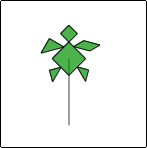
\includegraphics[width=3.0cm,trim=4 4 8 4,clip]{./images/disegnare/disegnare-2.png}
   \label{dis-2}
\end{figure}
\end{minipage} \hfill

\vskip 1cm

La tartaruga si è mossa tracciando una linea; è così che si disegna dando comandi alla tartaruga.
Scriviamo ora le seguenti istruzioni:

\vskip 1cm

\begin{scriptsize}
\begin{minipage}{0.45\textwidth}
\begin{itemize}[itemsep=-3pt,parsep=2pt]
\item[] \hspace{0.5cm} HOME 
\item[] \hspace{0.5cm} FORWARD 100
\item[] \hspace{0.5cm} \textbf{RIGHT 90}
\item[] \hspace{0.5cm} FORWARD 50
\item[] \hspace{0.5cm} \textbf{RIGHT 90}
\item[] \hspace{0.5cm} FORWARD 50
\item[] \hspace{0.5cm} \textbf{RIGHT 90}
\item[] \hspace{0.5cm} FORWARD 50
\item[] \hspace{0.5cm} RIGHT \textbf{90} 
\item[] \hspace{0.5cm} 
\end{itemize}
\end{minipage}
\end{scriptsize}
\begin{minipage}{0.5\textwidth}
\begin{figure}[H]
   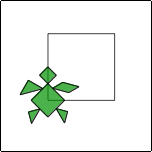
\includegraphics[width=3.0cm,trim=4 4 8 4,clip]{./images/disegnare/disegnare-3.png}
   \label{dis-3}
\end{figure}
\end{minipage} \hfill

\vskip 1cm

Abbiamo tracciato quattro lati, e alla fine di ogni lato abbiamo girato a destra di 90\degree, ottenendo così un quadrato.
  
Due parole sulla particolarità di LibreLogo.  La sequenza di istruzioni che abbiamo scritto è un frammento di codice, è software. L'abbiamo scritto in un particolare linguaggio, che è quello di Logo, ed è anche molto semplice, ma è software come qualsiasi altro. Di solito il software si scrive in appositi documenti mediante editori di testo semplice e si salvano in questo modo. Poi, si fanno eseguire al computer. I modi con qui si eseguono queste operazioni variano molto a seconda del tipo di linguaggio e di contesto. Oggi ci sono centinaia di linguaggi diversi che servono per gli scopi più disparati. La particolarità di LibreLogo è che il software si scrive in un documento e la tartaruga  "lavora " sul documento medesimo, lasciandovi la propria opera sotto forma di grafica, Così uno si ritrova insieme il codice e il risultato grafico prodotto da esso, in un unico documento. La grafica può essere selezionata con il mouse e, eventualmente, trasportata in contesti diversi. Ad esempio, le figure qui sopra le ho generate giocando con la tartaruga in un altro documento, poi ho selezionato le grafiche e le ho riportate qui. Un'altra notazione: un gruppo di istruzioni da fare funzionare in sequenza si chiama script, espressione che useremo diffusamente.

L'integrazione fra Logo e LibreOffice va oltre. È evidente che quando scriviamo il comando 

\vskip 1cm

\begin{scriptsize}
\begin{minipage}{1.0\textwidth}
\begin{itemize}[itemsep=-3pt,parsep=2pt]
\item[] \hspace{0.5cm} FORWARD 50  
\end{itemize}
\end{minipage}
\end{scriptsize}

\vskip 1cm

il numero 50 esprime la lunghezza del percorso che la tartaruga deve compiere. Puoi verificare subito cambiando il valore e guardando cosa fa la tartaruga. Ma cosa rappresenta quel 50?  Sono punti tipografici (point): 50 pt. Un punto sono 0.35 mm\footnote{La definizione precisa è: 1 pt = 1/72 polllici, dove 1 pollice = 25.4 mm. Quindi 1 pt = 2.54/72 = $.352\overline{7}$ mm}. LibreLogo capisce le unità di misura, si può scrivere 50, 50pt, 50mm, 50cm, 50in (inch: pollice), 50 " ( " sta per pollice). Ovviamente si tratta di lunghezze diverse. Usiamo per esempio i mm:

\vskip 1cm

\begin{scriptsize}
\begin{minipage}{0.45\textwidth}
\begin{itemize}[itemsep=-3pt,parsep=2pt]
\item[] \hspace{0.5cm} \textbf{CLEARSCREEN}
\item[] \hspace{0.5cm} HOME
\item[] \hspace{0.5cm} FORWARD \textbf{50mm}
\item[] \hspace{0.5cm} RIGHT 90
\item[] \hspace{0.5cm} FORWARD \textbf{50mm}
\item[] \hspace{0.5cm} RIGHT 90
\item[] \hspace{0.5cm} FORWARD \textbf{50mm}
\item[] \hspace{0.5cm} RIGHT 90
\item[] \hspace{0.5cm} FORWARD \textbf{50mm} 
\item[] \hspace{0.5cm} RIGHT 90     
\end{itemize}
\end{minipage}
\end{scriptsize}
\begin{minipage}{0.5\textwidth}
\begin{figure}[H]
   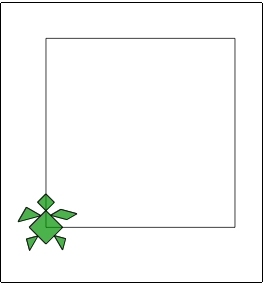
\includegraphics[width=5.0cm,trim=4 4 8 4,clip]{./images/disegnare/disegnare-4.png}
   \label{dis-4}
\end{figure}
\end{minipage} \hfill

\vskip 1cm

Il quadrato è ovviamente più grosso perché il precedente aveva il lato di 50 pt = 17.6 mm. 

Proviamo a complicare il disegno, immaginando di fare una casetta. La tartaruga si trova nel vertice in basso a sinistra e guarda in alto. Come prima cosa dobbiamo farla salire fino al vertice in alto a sinistra. Proviamo, e allo stesso tempo approfittiamo anche del fatto che le istruzioni possono essere raggruppate in una stessa riga, a seconda della convenienza:

\vskip 1cm

\begin{scriptsize}
\begin{minipage}{0.40\textwidth}
\begin{itemize}[itemsep=-3pt,parsep=2pt]
\item[] CLEARSCREEN             
\item[] HOME
\item[] FORWARD 50mm RIGHT 90
\item[] FORWARD 50mm RIGHT 90
\item[] FORWARD 50mm RIGHT 90
\item[] FORWARD 50mm RIGHT 90
\item[] FORWARD 50mm
\end{itemize}
\end{minipage}
\end{scriptsize}
\begin{minipage}{0.4\textwidth}
\begin{figure}[H]
   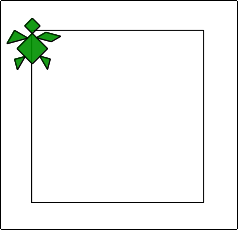
\includegraphics[width=5.0cm,trim=4 4 8 4,clip]{./images/disegnare/disegnare-5.png}
   \label{dis-5}
\end{figure}
\end{minipage} \hfill

\vskip 1cm

Non ci sono regole precise per raggruppare le istruzioni in una stessa riga. Il raggruppamento si può decidere in base alla comodità con cui si rilegge il codice. È importante facilitarsi la vita perché via via che il codice cresce può complicarsi rapidamente e tutti gli accorgimenti per renderlo più chiaro sono utili.

\vskip 1cm

\begin{minipage}{0.45\textwidth}
Ora dobbiamo costruire il tetto sulla casa. Facciamo questo appoggiando sul quadrato un triangolo equilatero, con la base coincidente con il lato superiore del quadrato. Essendo equilatero, anche gli altri due lati del triangolo saranno lunghi 50mm. Quindi per fare la falda sinistra del tetto la tartaruga dovrà spostarsi di 50mm ma deve prima cambiare direzione. Di quanto? Siccome gli angoli interni di un triangolo equilatero sono di 60\degree, la tartaruga dovrà deviare di 90\degree – 60\degree = 30\degree a destra. Arrivata in cima, disegnando la falda sinistra del tetto, dovrà girare a destra di 120\degree per poi disegnare la falda destra. Infine, girerà di 30\degree a destra per riallinearsi alla parete della casa.
\end{minipage}
\begin{minipage}{0.5\textwidth}
\begin{figure}[H]
   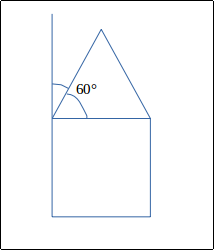
\includegraphics[width=6.5cm,trim=4 4 8 4,clip]{./images/disegnare/disegnare-6.png}
   \label{dis-6}
\end{figure}
\end{minipage} \hfill

\vskip 1cm

\begin{scriptsize}
\begin{minipage}{0.40\textwidth}
\begin{itemize}[itemsep=-3pt,parsep=2pt]
\item[] CLEARSCREEN             
\item[] HOME
\item[] FORWARD 50mm RIGHT 90
\item[] FORWARD 50mm RIGHT 90
\item[] FORWARD 50mm RIGHT 90
\item[] FORWARD 50mm RIGHT 90
\item[] FORWARD 50mm RIGHT 30
\item[] FORWARD 50mm RIGHT 120
\item[] FORWARD 50mm RIGHT 30
\end{itemize}
\end{minipage}
\end{scriptsize}
\begin{minipage}{0.4\textwidth}
\begin{figure}[H]
   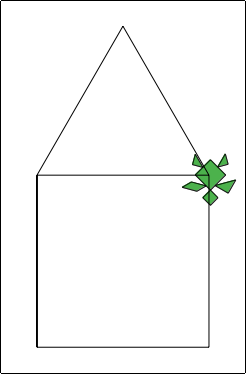
\includegraphics[width=5.0cm,trim=4 4 8 4,clip]{./images/disegnare/disegnare-7.png}
   \label{dis-7}
\end{figure}
\end{minipage} \hfill

\vskip 1cm

Supponiamo ora di voler disegnare una finestra nel mezzo della parete. Per fare questo è necessario introdurre due nuovi comandi - PENUP e PENDOWN – che consentono di muovere la tartaruga senza disegnare.

\vskip 1cm

\begin{scriptsize}
\begin{minipage}{0.40\textwidth}
\begin{itemize}[itemsep=-3pt,parsep=2pt]
\item[] CLEARSCREEN             
\item[] HOME
\item[] FORWARD 50mm RIGHT 90
\item[] FORWARD 50mm RIGHT 90
\item[] FORWARD 50mm RIGHT 90
\item[] FORWARD 50mm RIGHT 90
\item[] FORWARD 50mm RIGHT 30
\item[] FORWARD 50mm RIGHT 120
\item[] FORWARD 50mm RIGHT 120
\item[] \textbf{PENUP}
\item[] FORWARD 50mm/3 LEFT 90
\item[] FORWARD 50mm/3

dove abbiamo evidenziato in rosso il percorso fatto senza disegnare.
\end{itemize}
\end{minipage}
\end{scriptsize}
\begin{minipage}{0.4\textwidth}
\begin{figure}[H]
   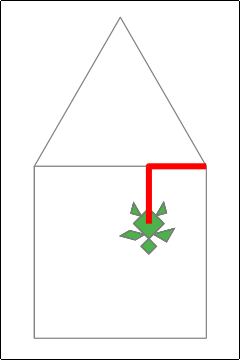
\includegraphics[width=5.0cm,trim=4 4 8 4,clip]{./images/disegnare/disegnare-8.png}
   \label{dis-8}
\end{figure}
\end{minipage} \hfill

\vskip 1cm

\begin{scriptsize}
\begin{minipage}{0.40\textwidth}
\begin{itemize}[itemsep=-3pt,parsep=2pt]
\item[] CLEARSCREEN             
\item[] HOME
\item[] FORWARD 50mm RIGHT 90
\item[] FORWARD 50mm RIGHT 90
\item[] FORWARD 50mm RIGHT 90
\item[] FORWARD 50mm RIGHT 90
\item[] FORWARD 50mm RIGHT 30
\item[] FORWARD 50mm RIGHT 120
\item[] FORWARD 50mm RIGHT 120
\item[] \textbf{PENUP}
\item[] FORWARD 50mm/3 LEFT 90
\item[] FORWARD 50mm/3
\item[] \textbf{PENDOWN}
\item[] FORWARD 50mm/3 RIGHT 90
\item[] FORWARD 50mm/3 RIGHT 90
\item[] FORWARD 50mm/3 RIGHT 90
\item[] FORWARD 50mm/3 RIGHT 90
\end{itemize}
\end{minipage}
\end{scriptsize}
\begin{minipage}{0.4\textwidth}
\begin{figure}[H]
   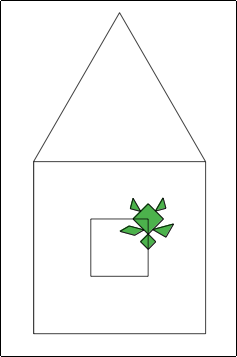
\includegraphics[width=5.0cm,trim=4 4 8 4,clip]{./images/disegnare/disegnare-9.png}
   \label{dis-9}
\end{figure}
\end{minipage} \hfill

\vskip 1cm

Proviamo ora ad arricchire ulteriormente il disegno, per esempio facendolo a colori.  

\vskip 1cm

\begin{scriptsize}
\begin{minipage}{0.40\textwidth}
\begin{itemize}[itemsep=-3pt,parsep=2pt]
\item[] CLEARSCREEN             
\item[] HOME
\item[] \textbf{PENCOLOR  "green "}
\item[] FORWARD 50mm RIGHT 90
\item[] FORWARD 50mm RIGHT 90
\item[] FORWARD 50mm RIGHT 90
\item[] FORWARD 50mm RIGHT 90
\item[] FORWARD 50mm RIGHT 30
\item[] \textbf{PENCOLOR  "red "}
\item[] FORWARD 50mm RIGHT 120
\item[] FORWARD 50mm RIGHT 120
\item[] PENUP
\item[] FORWARD 50mm/3
\item[] LEFT 90
\item[] FORWARD 50mm/3
\item[] PENDOWN
\item[] \textbf{PENCOLOR  "blue "}
\item[] FORWARD 50mm/3 RIGHT 90
\item[] FORWARD 50mm/3 RIGHT 90
\item[] FORWARD 50mm/3 RIGHT 90
\item[] FORWARD 50mm/3 RIGHT 90
\item[] \textbf{PENCOLOR  "gray "}
\end{itemize}
\end{minipage}
\end{scriptsize}
\begin{minipage}{0.4\textwidth}
\begin{figure}[H]
   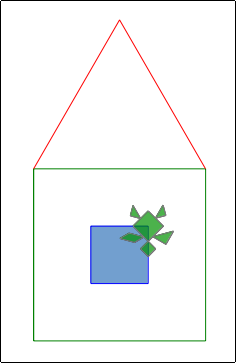
\includegraphics[width=5.0cm,trim=4 4 8 4,clip]{./images/disegnare/disegnare-10.png}
   \label{dis-10}
\end{figure}
\end{minipage} \hfill

\vskip 1cm

E perché non colorare anche l'interno?

\vskip 1cm

\begin{scriptsize}
\begin{minipage}{0.40\textwidth}
\begin{itemize}[itemsep=-3pt,parsep=2pt]
\item[] CLEARSCREEN            
\item[] HOME
\item[] FORWARD 50mm RIGHT 90
\item[] FORWARD 50mm RIGHT 90
\item[] FORWARD 50mm RIGHT 90
\item[] FORWARD 50mm RIGHT 90
\item[] FORWARD 50mm RIGHT 30
\item[] \textbf{FILLCOLOR  "yellow " FILL}
\item[] FORWARD 50mm RIGHT 120
\item[] FORWARD 50mm RIGHT 120
\item[] PENUP
\item[] FORWARD 50mm/3
\item[] LEFT 90
\item[] FORWARD 50mm/3
\item[] PENDOWN
\item[] \textbf{FILLCOLOR  "red " FILL}
\item[] FORWARD 50mm/3 RIGHT 90
\item[] FORWARD 50mm/3 RIGHT 90
\item[] FORWARD 50mm/3 RIGHT 90
\item[] FORWARD 50mm/3 RIGHT 90
\item[] \textbf{FILLCOLOR  "green " FILL}
\end{itemize}
\end{minipage}
\end{scriptsize}
\begin{minipage}{0.4\textwidth}
\begin{figure}[H]
   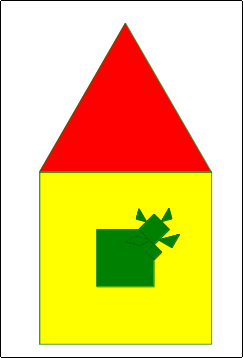
\includegraphics[width=5.0cm,trim=4 4 8 4,clip]{./images/disegnare/disegnare-11.png}
   \label{dis-11}
\end{figure}
\end{minipage} \hfill

\vskip 1cm

Anche in questo caso siamo ricorsi al raggruppamento delle istruzioni:
FILLCOLOR  "green " FILL. Con la prima si stabilisce il colore da usare
(FILLCOLOR  "green ") e con la seconda si procede a colorare la figura – viene
naturale inglobarle in una sola istruzione. 

L'istruzione FILL in realtà fa due cose: chiude una figura e la riempie di un
colore. Facciamo questa prova: 

\vskip 1cm

\begin{scriptsize}
\begin{minipage}{0.40\textwidth}
\begin{itemize}[itemsep=-3pt,parsep=2pt]
\item[] FORWARD 30mm RIGHT 90
\item[] FORWARD 30mm RIGHT 90
\end{itemize}
\end{minipage}
\end{scriptsize}
\begin{minipage}{0.4\textwidth}
\begin{figure}[H]
   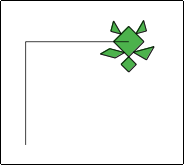
\includegraphics[width=5.0cm,trim=4 4 8 4,clip]{./images/disegnare/disegnare-12.png}
   \label{dis-12}
\end{figure}
\end{minipage} \hfill

\vskip 1cm

Così abbiamo disegnato una figura che non è chiusa. Volendo fare un triangolo potremmo far disegnare alla tartaruga il terzo lato. Alternativamente possiamo chiudere la figura con FILL, come abbiamo visto prima:

\vskip 1cm

\begin{scriptsize}
\begin{minipage}{0.40\textwidth}
\begin{itemize}[itemsep=-3pt,parsep=2pt]
\item[] FORWARD 30mm RIGHT 90
\item[] FORWARD 30mm RIGHT 90
\item[] FILL                  
\end{itemize}
\end{minipage}
\end{scriptsize}
\begin{minipage}{0.4\textwidth}
\begin{figure}[H]
   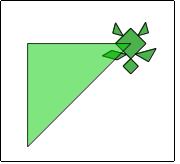
\includegraphics[width=5.0cm,trim=4 4 8 4,clip]{./images/disegnare/disegnare-13.png}
   \label{dis-13}
\end{figure}
\end{minipage} \hfill

\vskip 1cm

Così la figura è stata chiusa e colorata. Possiamo anche chiuderla senza
colorarla, usando l'istruzione \textbf{CLOSE}:

\vskip 1cm

\begin{scriptsize}
\begin{minipage}{0.40\textwidth}
\begin{itemize}[itemsep=-3pt,parsep=2pt]
\item[] FORWARD 30mm RIGHT 90
\item[] FORWARD 30mm RIGHT 90
\item[] CLOSE                  
\end{itemize}
\end{minipage}
\end{scriptsize}
\begin{minipage}{0.4\textwidth}
\begin{figure}[H]
   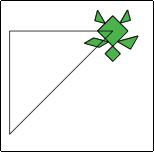
\includegraphics[width=5.0cm,trim=4 4 8 4,clip]{./images/disegnare/disegnare-14.png}
   \label{dis-14}
\end{figure}
\end{minipage} \hfill

\vskip 1cm

È interessante notare che, sia con FILL che con CLOSE la figura viene chiusa senza che la tartaruga  si sposti. Quindi se continuiamo ad aggiungere altri movimenti, questi prenderanno le mosse  da tale posizione della tartaruga, che negli esempi precedenti è rimasta volta verso il basso. Proviamo a mettere i due precedenti blocchi di codice uno dietro l'altro:

\vskip 1cm

\begin{scriptsize}
\begin{minipage}{0.40\textwidth}
\begin{itemize}[itemsep=-3pt,parsep=2pt]
\item[] FORWARD 30mm RIGHT 90
\item[] FORWARD 30mm RIGHT 90
\item[] FILL                  
\item[] FORWARD 30mm RIGHT 90
\item[] FORWARD 30mm RIGHT 90
\item[] CLOSE                  
\end{itemize}
\end{minipage}
\end{scriptsize}
\begin{minipage}{0.4\textwidth}
\begin{figure}[H]
   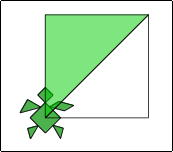
\includegraphics[width=5.0cm,trim=4 4 8 4,clip]{./images/disegnare/disegnare-15.png}
   \label{dis-15}
\end{figure}
\end{minipage} \hfill

\vskip 1cm

Dopo avere chiuso e colorato di verde il triangolo superiore, la tartaruga con le successive istruzioni di FORWARD procede a disegnare due lati del triangolo inferiore. L'istruzione CLOSE fa chiudere questo secondo triangolo senza colorarlo. 

E se uno volesse togliere la tartaruga una volta finito il disegno? Semplice: basta aggiungere alla fine l'istruzione \textbf{HIDETURTLE}. Prova! 

\subsection{I codici RGB per i colori}

Negli esempi precedenti abbiamo usato dei codici per esprimere i colori, per
esempio  "red " per indicare rosso. Si possono indicare così 24 colori: 

\vskip 1cm

\begin{figure}[H]
   \centering
   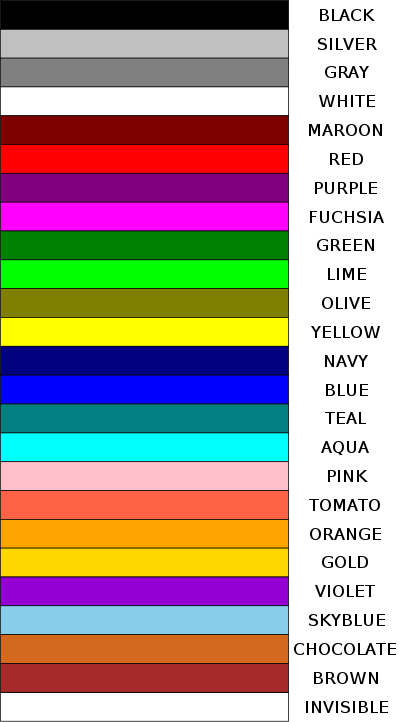
\includegraphics[width=8.0cm,trim=4 4 8 4,clip]{./images/disegnare/disegnare-16.png}
   \label{dis-16-a}
\end{figure}

In realtà i colori possibili sono molti di più. Questi possono essere espressi mediante il cosiddetto codice RGB, che sta per Red, Green, Blue. Nella grafica al computer i colori possono essere espressi come combinazione di tre colori fondamentali, che sono appunto rosso, verde e blu. Tutti gli altri possono essere espressi miscelando e dosando opportunamente questi tre colori fondamentali. Per fare questo si esprimono ile intensità dei singoli colori con un numero che va da 0 a 255 e si miscelano scrivendo ad esempio [255,0,0] per il rosso, [0,255,0] per il verde o [0,0,255] per il blu. Tutti gli altri colori si ottengono variando i valori all'interno delle parentesi. Con [0, 0, 0]  si ottiene il nero e con [255, 255, 255] il bianco. Poi questo tipo di codifica si utilizza in uno qualsiasi dei comandi che consentono di specificare il colore. Ad esempio

PENCOLOR [45, 88, 200]
FILLCOLOR [255, 200, 100]

Provate a giocare un po' con questi numeri per vedere che colori vengono fuori.

La tabella dei colori che abbiamo mostrato ha una stranezza: ci sono due elementi che hanno nome diverso ma il colore sembra lo stesso. Trovati? In realtà differiscono. ma per via di un quarto attributo, che è la trasparenza. Vediamo giocando un po'. 

Per facilitarci, anticipiamo un nuovo comando. Negli esempi precedenti noi abbiamo già disegnato un quadrato, utilizzando le istruzioni FORWARD e RIGHT, opportunamente combinate. In realtà, per disegnare le principali figure geometriche, in Logo esistono delle istruzioni preconfezionate, che ci aiutano a scrivere il codice in maniera più sintetica. Il quadrato è una di queste. Per fare un quadrato di 50 mm di lato si scrive:

\vskip 1cm

\begin{scriptsize}
\begin{minipage}{0.40\textwidth}
\begin{itemize}[itemsep=-3pt,parsep=2pt]
\item[] CLEARSCREEN
\item[] HOME
\item[] \textbf{SQUARE(30mm)}                            
\end{itemize}
\end{minipage}
\end{scriptsize}
\begin{minipage}{0.4\textwidth}
\begin{figure}[H]
   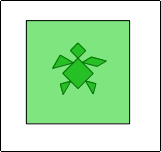
\includegraphics[width=5.0cm,trim=4 4 8 4,clip]{./images/disegnare/disegnare-17.png}
   \label{dis-16-b}
\end{figure}
\end{minipage} \hfill

\vskip 1cm

In questo modo la tartaruga disegna un quadrato e poi si piazza al centro con la testa rivolta in alto (il coloro non l'abbiamo determinato noi ma venuto  "automaticamente ", si dice che è il valore di default). Serviamoci allora di questa istruzione per disegnare prima un quadrato che coloriamo di rosso, poi spostiamoci un po' in basso e a destra, per disegnare un secondo quadrato, in modo che quest'ultimo si sovrapponga un poco al precedente, e poi lo coloriamo di bianco.

\vskip 1cm

\begin{scriptsize}
\begin{minipage}{0.40\textwidth}
\begin{itemize}[itemsep=-3pt,parsep=2pt]
\item[] CLEARSCREEN
\item[] HOME
\item[] FILLCOLOR [255, 0, 0]                                
\item[] SQUARE(50mm)
\item[] FORWARD -25mm
\item[] RIGHT 90                                             
\item[] FORWARD 25mm
\item[] FILLCOLOR [255, 255, 255]
\item[] SQUARE(50mm)                                         
\end{itemize}
\end{minipage}
\end{scriptsize}
\begin{minipage}{0.4\textwidth}
\begin{figure}[H]
   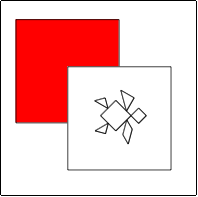
\includegraphics[width=5.0cm,trim=4 4 8 4,clip]{./images/disegnare/disegnare-18.png}
   \label{dis-17}
\end{figure}
\end{minipage} \hfill

\vskip 1cm

Bene, così il quadrato bianco si è sovrapposto a quello rosso. Un risultato prevedibile: i colori si sovrappongono perché sono opachi. Un pittore direbbe che  "coprono ". In realtà con i codici RGB in Logo si può assegnare un quarto parametro che è la  "trasparenza " che si vuole attribuire a quel certo colore, con la convenzione che un valore di 0 gli conferisce la completa opacità mentre il valore di 255 lo rende invece completamente trasparente. Con i valori compresi fra 0 e 255 si possono ottenere diversi livelli di trasparenza. Proviamo dunque a rendere trasparente il quadrato bianco, aggiungendo il quarto parametro uguale a 255:

\vskip 1cm

\begin{scriptsize}
\begin{minipage}{0.40\textwidth}
\begin{itemize}[itemsep=-3pt,parsep=2pt]
\item[] CLEARSCREEN
\item[] HOME
\item[] FILLCOLOR [255, 0, 0]                                
\item[] SQUARE(50mm)
\item[] FORWARD -25mm
\item[] RIGHT 90                                             
\item[] FORWARD 25mm
\item[] FILLCOLOR [255, 255, 255, 255]
\item[] SQUARE(50mm)                                        
\end{itemize}
\end{minipage}
\end{scriptsize}
\begin{minipage}{0.4\textwidth}
\begin{figure}[H]
   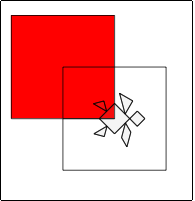
\includegraphics[width=5.0cm,trim=4 4 8 4,clip]{./images/disegnare/disegnare-19.png}
   \label{dis-18}
\end{figure}
\end{minipage} \hfill

\vskip 1cm

Il quadrato bianco è diventato trasparente. Se al posto di FILLCOLOR [255, 255, 255, 255] avessimo usato FILLCOLOR  "invisible " allora avremmo ottenuto lo stesso risultato. Ecco in cosa consiste la differenza fra il colore  "white " (bianco) e  "invisible ", invisibile, nella tabella che abbiamo visto all'inizio. 
Un'ultima annotazione. A guardare bene, si vede che in questi disegni ci ritroviamo con la tartaruga di colori diversi. Di fatto, la tartaruga viene colorata con lo stesso colore che abbiamo selezionato per riempire l'ultima figura disegnata, magari con una trasparenza diversa. Dopo avere disegnato il quadrato verde chiaro, la tartaruga è venuta verde un po' più scuro. Dopo il quadrato bianco è venuta grigio chiaro e dopo il colore invisibile e venuta grigio scuro. Questo è un comportamento che comunque non inficia i risultati che vogliamo ottenere perché qualora volessimo usare in qualche maniera le grafiche che produciamo, alla fine non avremo da fare altro che aggiungere l'istruzione HIDETURTLE.

\subsection{Altri comandi}

on i comandi di base che abbiamo visto fin qui è possibile produrre una gran quantità di grafiche. In Logo sono tuttavia disponibili dei comandi che consentono di abbreviare il disegno di alcune forma base. Abbiamo già anticipato l'istruzione SQUARE che consente di costruire un quadrato in un sol colpo. Le altre sono RECTANGLE, CIRCLE e ELLIPSE, che servono a costruire rispettivamente rettangoli, cerchi e ellissi.
Proviamo i seguenti comandi:

\vskip 1cm

\begin{scriptsize}
\begin{scriptsize}
\begin{minipage}{0.40\textwidth}
\begin{itemize}[itemsep=-3pt,parsep=2pt]
\item[] CLEARSCREEN
\item[] HOME
\item[] SQUARE 50                               
\item[] CIRCLE 50                                       
\end{itemize}
\end{minipage}
\end{scriptsize}
\end{scriptsize}
\begin{minipage}{0.4\textwidth}
\begin{figure}[H]
   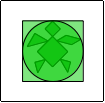
\includegraphics[width=3.0cm,trim=4 4 8 4,clip]{./images/disegnare/disegnare-20.png}
   \label{dis-19}
\end{figure}
\end{minipage} \hfill

\vskip 1cm

Si vede come l'effetto di disegnare due figure in sequenza sia quello di sovrapporle facendone coincidere il centro di simmetria e come la tartaruga si riposizioni sempre su tale centro. Si capisce anche come l'argomento\footnote{Con "argomento" si intende il valore che un comando richiede per essere effettuato. Gli argomenti possono essere anche più di uno – vedremo degli esempi. } del comando SQUARE rappresenti il lato del quadrato e quello del comando CIRCLE il diametro del cerchio che vogliamo costruire.

\vskip 1cm

\begin{minipage}{0.40\textwidth}
Prova a esercitarti con i comandi SQUARE e CIRCLE, per esempio costruendo la locomotiva qui accanto. Puoi esercitarti a rispettare delle proporzioni date, come quelle in questo esempio, dove il lato del quadrato più grande è due o tre volte quelli dei quadrati più piccoli e il diametro dei cerchi è pari al lato del quadrato più piccolo. A pagina nuova c'è una possibile soluzione, ma prima prova da solo. 
\end{minipage}
\begin{minipage}{0.4\textwidth}
\begin{figure}[H]
   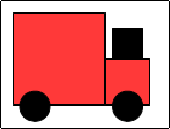
\includegraphics[width=5.0cm,trim=4 4 8 4,clip]{./images/disegnare/disegnare-21.png}
   \label{dis-20}
\end{figure}
\end{minipage} \hfill

\vskip 1cm

Una cosa importante di cui rendersi conto con il codice è che lo stesso obiettivo può essere conseguito in tanti modi diversi. Non esiste un criterio assoluto per stabilire quale sia il procedimento migliore. Quindi non esiste un'unica  "risposta giusta ". Un procedimento può essere meglio di un altro sotto un certo punto di vista: chiarezza del codice scritto, velocità di esecuzione, memoria totale impiegata dal codice, gestione di eventuali risorse ecc. Può succedere che un ottimo codice sotto uno di questi punti vista risulti pessimo sotto un altro.  

\newpage

\begin{scriptsize}
\begin{minipage}{0.40\textwidth}
\begin{itemize}[itemsep=-3pt,parsep=2pt]
\item[] COLOR  "red " 
\item[] SQUARE 60 
\item[] PENUP BACK 15 RIGHT 90 FORWARD 45                      
\item[] LEFT 90 PENDOWN 
\item[] SQUARE 30 
\item[] PENUP FORWARD 25 PENDOWN 
\item[] FILLCOLOR  "black "                      
\item[] SQUARE 20 
\item[] PENUP BACK 40 PENDOWN 
\item[] CIRCLE 20                                              
\item[] PENUP LEFT 90 FORWARD 60 PENDOWN 
\item[] CIRCLE 20
\item[] HIDETURTLE                                            
\end{itemize}
\end{minipage}
\end{scriptsize}

\vskip 1cm

Il quadrato e il cerchio hanno bisogno di un solo parametro per essere specificati. Invece, il rettangolo e l'ellisse hanno bisogno di due parametri. Nel caso del rettangolo i due parametri sono le lunghezze del lato lungo e del lato corto. L'istruzione per costruire un rettangolo è la seguente:

\textbf{RECTANGLE [60,40]}

Questo comando produce un rettangolo largo 60 punti e altro 40. Rispetto ai casi del quadrato de del cerchio questo comando ha un'altra particolarità: in questo caso, per fornire i due parametri necessari, si è ricorsi alla scrittura \textbf{[60,40]}. Questa è una  "lista " di valori. Si tratta di un modo per considerare un insieme di valori come un'unica cosa, una lista appunto, e il modo per ottenere questo effetto è quello di elencare i valori separandoli con le virgole e richiudendo tutto fra parentesi quadre. Le liste possono servire in varie circostanze, non solo in questo caso, ma vedremo successivamente come.
\textbf{Esercizio}: prova a realizzare un figura come questa qui sotto

\vskip 1cm

\begin{figure}[H]
   \centering
   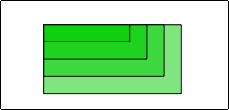
\includegraphics[width=4.0cm,trim=4 4 8 4,clip]{./images/disegnare/disegnare-22.png}
   \label{dis-21}
\end{figure}

\vskip 1cm

Anche in questo caso, prova da solo. Poi, a pagina nuova puoi vedere un possibile modo per risolverlo.

\pagebreak

\vskip 1cm
\begin{scriptsize}
\begin{minipage}{1.0\textwidth}
\begin{itemize}[itemsep=-3pt,parsep=2pt]
\item[] RECTANGLE [40mm, 20mm]
\item[] PENUP FORWARD 2,5mm LEFT 90
\item[] FORWARD 2,5mm RIGHT 90 PENDOWN   
\item[] RECTANGLE [35mm, 15mm]
\item[] PENUP FORWARD 2,5mm LEFT 90
\item[] FORWARD 2,5mm RIGHT 90 PENDOWN
\item[] RECTANGLE [30mm, 10mm]
\item[] PENUP FORWARD 2,5mm LEFT 90      
\item[] FORWARD 2,5mm RIGHT 90 PENDOWN
\item[] RECTANGLE [25mm, 5mm]
\item[] HIDETURTLE                      
\end{itemize}
\end{minipage}
\end{scriptsize}

\vskip 1cm

Un'altra figura che può tornare utile è l'ellisse. Detto nel più semplice dei modi l'ellisse è un cerchio schiacciato. È perfettamente nello spirito della geometria della Tartaruga quello di aiutarsi con riferimenti ad attività fisiche: probabilmente il miglior modo di usare le tecnologie moderne è di continuare ad utilizzare quelle tradizionali, integrando al meglio le une con le altre. Niente di meglio qui che farsi aiutare da Emma Castelnuovo\cite{Castelnuovo}, in un suo brano dove l'ellisse emerge studiando la classe di triangoli isoperimetrici con uguale base. Riportiamo il brano per intero, al fine di rispettare l'intento didattico di Emma, che è di valore:

\begin{quote}
Sempre un argomento di matematica, quale lo studio dei triangoli isoperimetrici con ugual base, porta a osservare quello che abbiamo sotto gli occhi. 

Il materiale è, anche questa volta, un pezzo di spago.

Per costruire dei triangoli di uguale base e uguale perimetro facciamo così: fissiamo due chiodi – siano A e B – su un tavolo su cui è disteso un foglio di carta; AB sarà la base dei nostri triangoli. Leghiamo poi gli estremi di un pezzo di spago ai due chiodi, tenendo presente che lo spago deve essere più lungo del tratto AB. Facciamo in modo, valendoci di una matita, che lo spago resti sempre ben teso e... lasciamoci guidare dalla matita.

Questa, guidata dallo spago, disegnerà sul foglio una curva a forma di ovale: è un'ellisse. I punti A e B si chiamano fuochi dell'ellisse. Dunque: i vertici dei triangoli isoperimetrici e di uguale base si trovano su un'ellisse.

Un problema di geometria ci ha condotti al disegno dell'ellisse. Con lo stesso pezzo di spago possiamo costruire un'ellisse più o meno  "schiacciata ", a seconda della distanza fra i punti A e B. Si può ottenere anche un cerchio, se i due punti coincidono: il cerchio, infatti, è un'ellisse particolare.    

L'ellisse, dopo averla incontrata in problemi di geometria, la ritroviamo per la strada, quando la  "calpestiamo " (perché un disco segnaletico dà, come ombra, un'ellisse. Nella nostra vita convulsa raramente ci soffermiamo a osservare l'ombra di un oggetto data dai raggi del soleo da una lampadina. Ma ecco che ora un'attività di geometria ci sollecita a guardare di più ed è proprio il confronto fra l'effetto-ombra dato dai raggi del sole e quello dato da una lampada puntiforme che stimola la nostra facoltà di osservazione. 

Guardiamo, ad esempio, due matite disposte in verticale su un tavolo. Se vengono illuminate dal sole accade che anche le ombre sono parallele; se invece è una lampada che le illumina le ombre si divaricano.

Da qui lo studio matematico delle trasformazioni affini e delle trasformazioni proiettive, fino ad arrivare alla prospettiva, all'arte, a come si guarda un quadro, alla storia.

È un piccolo problema di geometria che ha stimolato a osservare e a... guardarsi intorno.

\vskip 1cm

\begin{figure}[H]
   \centering
   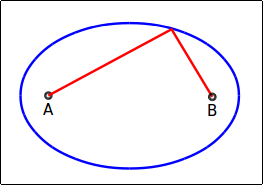
\includegraphics[width=8.0cm,trim=4 4 8 4,clip]{./images/disegnare/disegnare-23.png}
   \label{dis-22}
\end{figure}

\vskip 1cm

\end{quote}

In LibreLogo l'ellisse si disegna con il comando

\vskip 1cm

\begin{scriptsize}
\begin{minipage}{0.40\textwidth}
\begin{itemize}[itemsep=-3pt,parsep=2pt]
\item[] \textbf{ELLIPSE[40, 20]}
\end{itemize}
\end{minipage}
\end{scriptsize}

\vskip 1cm

L'ellisse ovviamente non ha un diametro fisso, come il cerchio. Per questo per essere definita richiede due parametri che sono i due assi, maggiore e minore. Nell'esempio l'ellisse ha l'asse maggiore uguale a 60 punti e il minore uguale a 40 punti. È possibile combinare le varie forme e aggiustare i loro parametri per ottenere una varietà di effetti. Per esempio un cerchio inscritto in un quadrato si può ottenere anche partendo dalle istruzioni per disegnare rettangoli e ellissi:

\vskip 1cm

\begin{scriptsize}
\begin{minipage}{0.40\textwidth}
\begin{itemize}[itemsep=-3pt,parsep=2pt]
\item[] RECTANGLE [60, 60] 
\item[] ELLIPSE [60, 60]   
\end{itemize}
\end{minipage}
\end{scriptsize}

\vskip 1cm

Prova a fare una figura come questa:

\vskip 1cm

\begin{figure}[H]
   \centering
   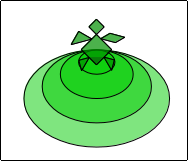
\includegraphics[width=4.0cm,trim=4 4 8 4,clip]{./images/disegnare/disegnare-24.png}
   \label{dis-23}
\end{figure}

\vskip 1cm
\pagebreak

Risposta possibile:

\vskip 1cm

\begin{scriptsize}
\begin{minipage}{0.40\textwidth}
\begin{itemize}[itemsep=-3pt,parsep=2pt]
\item[] ELLIPSE [120, 80] 
\item[] PENUP FORWARD 10 PENDOWN
\item[] ELLIPSE [90, 60]         
\item[] PENUP FORWARD 10 PENDOWN
\item[] ELLIPSE [60, 40] 
\item[] PENUP FORWARD 10 PENDOWN
\item[] ELLIPSE [30, 20] 
\item[] PENUP FORWARD 10 PENDOWN 
\end{itemize}
\end{minipage}
\end{scriptsize}

\vskip 1cm

Queste istruzioni consentono di usare anche altri parametro per ottenere delle varianti di rettangoli e ellissi. Nel caso dei rettangoli è possibile aggiustare un terzo parametro in maniera da arrotondare i vertici:

\vskip 1cm

\begin{scriptsize}
\begin{minipage}{0.40\textwidth}
\begin{itemize}[itemsep=-3pt,parsep=2pt]
\item[] RECTANGLE [60, 50, \textbf{10}]
\end{itemize}
\end{minipage}
\end{scriptsize}
\begin{minipage}{0.4\textwidth}
\begin{figure}[H]
   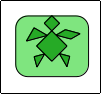
\includegraphics[width=3.0cm,trim=4 4 8 4,clip]{./images/disegnare/disegnare-25.png}
   \label{dis-24}
\end{figure}
\end{minipage} \hfill

\vskip 1cm

Supponiamo ora che un amico ci abbia appena detto di questa possibilità ma che altro non si ricordi. Si può controllare la  "rotondità " dei vertici? Probabilmente con quel terzo parametro, che l'amico ci ha detto potevamo fissare al valore di 10, ma come funziona? Questo è un ottimo esempio per mettere in luce lo strumento fondamentale di chi sviluppa software: la sperimentazione. Ecco, in questo caso, potremmo provare a fare dei tentativi, che potremmo (è solo una delle innumerevoli possibilità) sintetizzare così:

\vskip 1cm

\begin{scriptsize}
\begin{minipage}{0.40\textwidth}
\begin{itemize}[itemsep=-3pt,parsep=2pt]
\item[] FILLCOLOR  "invisible " 
\item[] PENCOLOR  "green " 
\item[] RECTANGLE [200, 150, 0] 
\item[] PENCOLOR  "black " 
\item[] RECTANGLE [200, 150, 10] 
\item[] RECTANGLE [200, 150, 20] 
\item[] RECTANGLE [200, 150, 30] 
\item[] RECTANGLE [200, 150, 40] 
\item[] RECTANGLE [200, 150, 50] 
\item[] RECTANGLE [200, 150, 60] 
\item[] RECTANGLE [200, 150, 70] 
\item[] RECTANGLE [200, 150, 80] 
\item[] RECTANGLE [200, 150, 90] 
\item[] RECTANGLE [200, 150, 100] 
\item[] PENCOLOR  "red " 
\item[] ELLIPSE [200,150]          
\end{itemize}
\end{minipage}
\end{scriptsize}
\begin{minipage}{0.4\textwidth}
\begin{figure}[H]
   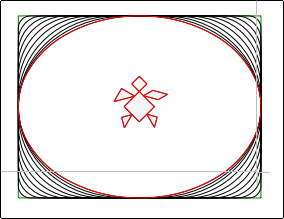
\includegraphics[width=5.0cm,trim=4 4 8 4,clip]{./images/disegnare/disegnare-26.png}
   \label{dis-25}
\end{figure}
\end{minipage} \hfill

\vskip 1cm
 
In questo modo ci siamo fatti un'idea di come possiamo controllare i rettangoli arrotondati. Ci siamo anche resi conto che, giocando con il terzo parametro, possiamo andare dal caso limite del rettangolo normale all'ellisse vera e propria.
Vediamo ora le varianti possibili per l'istruzione ELLIPSE.

\vskip 1cm

\begin{figure}[H]
   \centering
   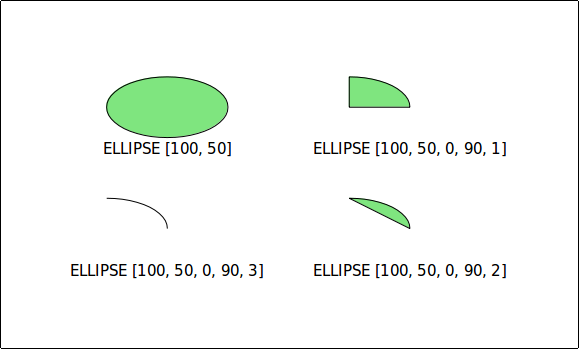
\includegraphics[width=10.0cm,trim=8 8 8 8,clip]{./images/disegnare/disegnare-27.png}
   \label{dis-26}
\end{figure}

\vskip 1cm

Nell'istruzione ELLIPSE possiamo quindi utilizzare 3 parametri aggiuntivi, che servono a disegnare solo un settore dell'ellisse. I primi due rappresentano l'angolo iniziale e finale, espressi in gradi, che delimitano il settore. Nell'esempio sopra, avendo scelto 0 e 90 abbiamo imposto di disegnare il primo quadrante dell'ellisse. Il quarto parametro stabilisce se si vuole disegnare un settore di ellisse (1), un segmento di ellisse (2) oppure giusto un arco (3).

\subsection{Le variabili} \label{sec:variabili}

 Le istruzioni che abbiamo visto sin'ora consentono di fare molte cose: abbiamo imparato a muovere la tartaruga in ogni parte del foglio, a farla disegnare o meno, abbiamo visto come controllare il colore del tratto e il riempimento delle figure. Si potrebbe avere la sensazione che per produrre grafica non occorra altro. Invece abbiamo solo scalfito la superficie delle potenzialità di un linguaggio di programmazione, anche se questo ha finalità esclusivamente didattiche, come nel caso di Logo e dei suoi derivati. Introdurremo via via le caratteristiche più importanti. Fra queste la prima, che ci serve subito per poter andare avanti,  è il concetto di  "variabile ". Fin qui abbiamo usato varie istruzioni che richiedono degli  "argomenti ". L'argomento è il valore che un'istruzione può richiedere per poter essere eseguita. Ad esempio l'istruzione FORWARD non avrebbe senso senza un argomento che rappresenti la distanza che la tartaruga deve percorrere. L'espressione FORWARD 50  significa che la tartaruga deve muoversi in avanti di 50 punti; 50 è il valore dell'argomento. Vi sono anche istruzioni che richiedono più di un argomento, è per esempio il caso di RECTANGLE e ELLIPSE. In ogni caso, in tutti gli esempi visti precedentemente abbiamo sempre usato argomenti numerici per tutte le istruzioni. In realtà, tutti i linguaggi consentono di servirsi di un'importante generalizzazione che consiste nell'uso delle  "variabili ". Si tratta di nomi simbolici ai quali possono essere assegnati vali numerici a piacimento. Proviamo ad eseguire il seguente codice:

\vskip 1cm

\begin{scriptsize}
\begin{minipage}{0.40\textwidth}
\begin{itemize}[itemsep=-3pt,parsep=2pt]
\item[] CLEARSCREEN
\item[] HOME
\item[] 
\item[] LATO = 100
\item[] ANGOLO = 90
\item[] 
\item[] FORWARD LATO
\item[] LEFT ANGOLO
\item[] FORWARD LATO
\item[] LEFT ANGOLO
\item[] FORWARD LATO
\item[] LEFT ANGOLO
\item[] FORWARD LATO
\item[] HIDETURTLE    
\end{itemize}
\end{minipage}
\end{scriptsize}
\begin{minipage}{0.4\textwidth}
\begin{figure}[H]
   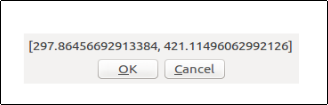
\includegraphics[width=3.0cm,trim=4 4 8 4,clip]{./images/disegnare/disegnare-28.png}
   \label{dis-27}
\end{figure}
\end{minipage} \hfill

\vskip 1cm

Abbiamo disegnato un quadrato, ma invece di utilizzare direttamente il valore 100 come argomento delle istruzioni FORWARD, abbiamo prima assegnato il valore 100 alla variabile di nome  "LATO " e poi abbiamo utilizzato questa come argomento di tutte le istruzioni FORWARD. È evidente quale possa essere l'utilità di questo metodo: supponiamo che non sia soddisfatto delle dimensioni di questo quadrato e che voglia provare altri valori del lato. Ebbene, non ho altro che da cambiare il valore 100 nell'istruzione LATO = 100, cambiandola per esempio con LATO = 150. Prova a sperimentare! Puoi anche cambiare il valore di ANGOLO, sperimentando con valori diversi... 
Coloro che hanno studiato i primi rudimenti dell'algebra, avranno certamente riconosciuto il concetto di variabile, che in quella disciplina si utilizza ampiamente per eseguire calcoli simbolici. Si ricorderanno anche che il concetto di variabile si declina in vari modi, per esprimere quantità che si considerano effettivamente variabili – ad esempio una variabile dipendente in funzione di altre variabili indipendenti – poi quantità che si assumono costanti, infine quantità che assumono il significato di parametri, che sono come costanti che possiamo avere interesse a cambiare di tanto in tanto. In ogni caso tutte queste quantità vengono rappresentate in maniera simbolica. In realtà, coloro che hanno poi avuto modo di approfondire lo studio dell'algebra, sanno che il  concetto di variabile è passibile di tutta una serie di generalizzazioni. Niente paura, questo non è un corso di matematica sottobanco, o forse un po' sì: in fin dei conti Logo rappresenta l'anelito di Seymour Papert di rendere la matematica più accessibile. Ma ciò che proponiamo qui non richiede doti o attitudini particolari. Introduciamo solo una delle generalizzazioni possibili, che ci servirà immediatamente. La generalizzazione che proponiamo attiene al concetto di posizione della tartaruga nel foglio. La posizione lungo una linea è determinata da un semplice numero – ad esempio la posizione lunga una strada:  "si segnalano lavori in corso al Km 287... ". Diverso è il caso della posizione su di una superficie. In un  navigatore satellitare, che oggi tutti conoscono, si può dare anche la posizione in termini geografici, ma questa deve essere somministrata mediante due valori: la latitudine e la longitudine, che designano il parallelo terrestre la prima e il meridiano la seconda. Per affondare una nave nel gioco della battagli navale occorre fornire due coordinate, per esempio b7, dove  "b rappresenta la colonna e 7 la riga. Allo stesso modo si identificano le celle di un foglio di lavoro, e via dicendo. Anche alla nostra tartaruga occorrono due valori numerici per identificare una posizione precisa nel foglio, che possiamo immaginare come la x e la y della tartaruga nello spazio della pagina. Ebbene, il modo per esprimere questo concetto nel mondo della tartaruga (ma non solo!) è il seguente:

\vskip 1cm

\begin{scriptsize}
\begin{minipage}{0.40\textwidth}
\begin{itemize}[itemsep=-3pt,parsep=2pt]
\item[] P=[200, 300]
\item[] PRINT P
\end{itemize}
\end{minipage}
\end{scriptsize}

\vskip 1cm

Se si esegue questo codice, LibreLogo stampa il  "valore " [200, 300]. Ovviamente abbiamo scelto questi numeri in maniera del tutto arbitraria, giusto per fare un esempio. Lo scopo è quello di mostrare come si rappresenta in maniera simbolica una posizione, che in realtà è espressa mediante un insieme di due numeri. Nell'algebra si dice che questo tipo di variabile è un  "vettore ". C'è anche un modo per  "isolare " i singoli elementi all'interno di un vettore. La cosa si descrive subito con questo esempio:

\vskip 1cm

\begin{scriptsize}
\begin{minipage}{0.40\textwidth}
\begin{itemize}[itemsep=-3pt,parsep=2pt]
\item[] P=[200, 300]
\item[] PRINT P
\item[] PRINT P[0]
\item[] PRINT P[1]
\end{itemize}
\end{minipage}
\end{scriptsize}

\vskip 1cm

Se si esegue questo frammento di codice, prima viene stampato  "valore " [200, 300], poi il valore 200, quindi 300. Da qui si capisce che con P [0] si ottiene il primo elemento del vettore posizione, che contiene il numero 200, e con P [1] il secondo elemento, che contiene il numero 300.
Ecco, questo è quanto dovrebbe bastare per andare a vedere com'è che si può controllare con ancora maggiore agilità la posizione della tartaruga nel foglio. 

\subsection{Lo spazio della pagina} \label{se:spazio-pagina}

Abbiamo già visto vari comandi per muovere la tartaruga ma sono tutti finalizzati al disegno. È vero che si possono fare i movimenti con la  "penna alzata " (comando PENUP) ma può essere utile  "saltare " direttamente in una posizione qualsiasi del foglio, oppure puntare in una direzione precisa.  Si tratta, in altre parole, di scegliere una posizione o una direzione in termini assoluti e non in modo relativo, rispetto alla posizione e direzione corrente, come si fa per esempio con istruzioni del tipo FORWARD oppure LEFT. Qui sorge la necessità di utilizzare dei  riferimenti spaziali assoluti che sono una coppia di coordinate per la posizione nel foglio e un angolo per la direzione. Per sapere come funzionano tali riferimenti introduciamo e usiamo subito due nuove istruzioni: \textbf{POSITION}  e \textbf{HEADING}. Inoltre, ci è utile anche l'istruzione \textbf{PRINT}, per conoscere il valore corrente della posizione e della direzione. Infatti i due comandi \textbf{POSITION} e \textbf{HEADING}, si possono usare con e senza parametri. Quando si usano senza parametri allora questi forniscono i valori correnti. Infatti, se apro un nuovo documento in Writer e faccio eseguire il comando

\vskip 1cm

\begin{scriptsize}
\begin{minipage}{1.0\textwidth}
\begin{itemize}[itemsep=-3pt,parsep=2pt]
\item[] \textbf{PRINT POSITION}
\end{itemize}
\end{minipage}
\end{scriptsize}

\vskip 1cm

si ottiene la seguente risposta:

\vskip 1cm

\begin{figure}[H]
   \centering
   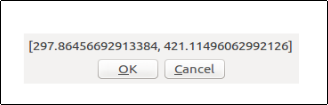
\includegraphics[width=10.0cm,trim=8 8 8 8,clip]{./images/disegnare/disegnare-28.png}
   \label{dis-28}
\end{figure}

\vskip 1cm

I due numeri fra parentesi rappresentano le coordinate x e y della posizione nello spazio della pagina: 298 e 421\footnote{Abbiamo arrotondato i due numeri a quattro cifre significative, che sono adeguate a determinare la posizione nel foglio, ai nostri fini. Nella nota successiva diamo una breve spiegazione dell'unità di misura impiegata per questi numeri.} rispettivamente. Dal momento che abbiamo appena aperto il documento e che all'inizio la tartaruga viene piazzata al centro, possiamo assumere che queste coordinate rappresentino il centro della pagina. Tuttavia, per avere il controllo completo della situazione occorre conoscere precisamente l'estensione dello spazio dell'immagine.  Ebbene, le coordinate dell'angolo superiore sinistro sono [0, 0], dove il primo numero rappresenta la coordinata x e il secondo la y, mentre quelle dell'angolo inferiore destro si ottengono stampando il valore della variabile speciale \textbf{PAGESIZE}, che LibreLogo utilizza per conservare le dimensioni della pagina. In questo momento la mia versione di Writer è predisposta per pagine di dimensioni A4 e, conseguentemente, eseguendo l'istruzione 

\vskip 1cm

\begin{scriptsize}
\begin{minipage}{1.0\textwidth}
\begin{itemize}[itemsep=-3pt,parsep=2pt]
\item[] \textbf{PRINT PAGESIZE}
\end{itemize}
\end{minipage}
\end{scriptsize}

\vskip 1cm

otteniamo:

\vskip 1cm

\begin{figure}[H]
   \centering
   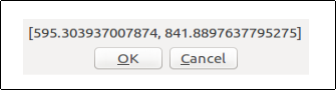
\includegraphics[width=10.0cm,trim=8 8 8 8,clip]{./images/disegnare/disegnare-29.png}
   \label{dis-29}
\end{figure}

\vskip 1cm

Questi numeri, arrotondati, 596 e 842, rappresentano le dimensioni di un foglio A4 espressi in  "punti " alla densità di 72 DPI/footnote{L'acronimo DPI sta per dots per inch: punti per pollice. Il valore di DPI dipende dal supporto fisico su cui si intende che un'immagine debba essere rappresentata. Poiché un pollice vale 2.54 cm, la densità di 72 DPI corrisponde a 72/2.54 = 28.3 punti per cm, o 2.83 punti per mm; giusto per avere un riferimento a noi più famigliare. Quando in Writer si sceglie l'unità di misura  "punti " (anziché cm o pollici), questi si riferiscono alla densità di 72 DPI appena citata. In Writer, l'unità di misura si può cambiare con la voce di menu Tools->Options->LibreOffice Writer->General. Si può scegliere fra mm, cm, pollici, pica, punti.}. In mm risultano 210 e 297 mm. Riassumiamo la situazione con la seguente figura.

\vskip 1cm

\begin{figure}[H]
   \centering
   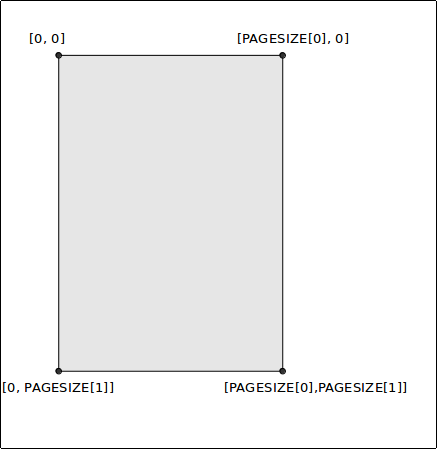
\includegraphics[width=10.0cm,trim=8 8 8 8,clip]{./images/disegnare/disegnare-30.png}
   \label{dis-30}
\end{figure}

\vskip 1cm

Tutte le volte che vogliamo utilizzare le posizioni assolute possiamo fare riferimento a questo schema che ci fornisce l'orientamento del sistema di riferimento sul foglio e le sue dimensioni. Nella tabella successiva vediamo i valori numerici corrispondenti:

\begin{center}
%\begin{tabular}{| >{\centering\arraybackslash}m{1in} | >{\centering\arraybackslash}m{1in} |}
\begin{tabular}{| l | l |}
\hline
[0, 0] & [0, 0] \\ \hline
[PAGESIZE[0], 0]  & [596, 0] \\ \hline 
[0, PAGESIZE[1]]  &     [0, 842]   \\ \hline 
[PAGESIZE[0], PAGESIZE[1]]  & [596, 842]   \\ \hline 
\end{tabular}
\end{center}

Riallacciandosi al paragrafo precedente, PAGESIZE è una variabile, una variabile che all'interno di LibreLogo è trattata come una costante perché contiene le dimensioni della pagina. Inoltre è quel particolare tipo di variabile che si chiama vettore, perché composta da più elementi, precisamente due, le due dimensioni della pagina: PAGESIZE[0] è la larghezza e PAGESIZE[1] la lunghezza.
Come facciamo dunque per spedire la tartaruga in una posizione precisa?

\vskip 1cm

\begin{figure}[H]
   \centering
   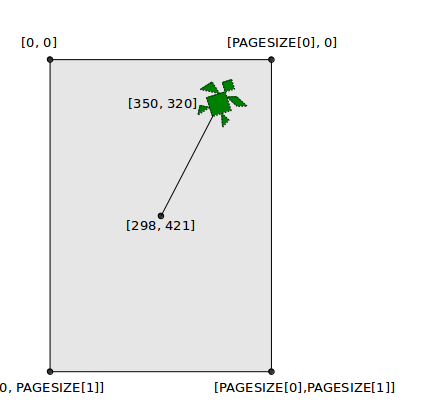
\includegraphics[width=10.0cm,trim=8 8 8 8,clip]{./images/disegnare/disegnare-31.png}
   \label{dis-31}
\end{figure}

\vskip 1cm

Con l'istruzione \textbf{POSITION [350, 320]} la tartaruga si dirige direttamente al punto di coordinate \textbf{POSITION [[350,320]}, a partire dal punto dive si trova, in questo caso dal centro della pagina.

Come possiamo usare l'istruzione POSITION per controllare la posizione, in modo analogo possiamo utilizzare l'istruzione HEADING per controllare la direzione in cui punta la tartaruga. Invocando l'istruzione HEADING senza alcun parametro si ottiene la posizione corrente. Utilizzando invece un parametro, per esempio HEADING [30], si impone alla tartaruga di ruotare di 30\degree. Nella figura seguente si mostra l'orientamento del sistema di riferimento.

\vskip 1cm

\begin{figure}[H]
   \centering
   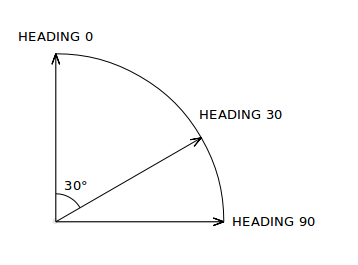
\includegraphics[width=10.0cm,trim=8 8 8 8,clip]{./images/disegnare/disegnare-32.png}
   \label{dis-32}
\end{figure}

\vskip 1cm

Quando si apre un documento nuovo, oppure dopo l'istruzione HOME, la tartaruga punta verso il lato superiore del foglio, e questa direzione corrisponde a 0\degree.

\subsection{Altri comandi grafici}

È possibile controllare anche altri aspetti del disegno, oltre al colore.

\subsubsection{PENWIDTH (spessore tratto)}

Con il comando \textbf{PENWIDTH} si determina lo spessore del tratto:


\vskip 1cm

\begin{figure}[H]
   \centering
   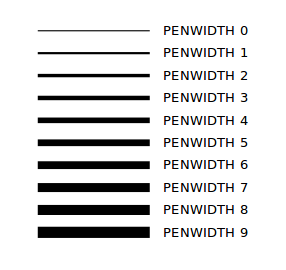
\includegraphics[width=10.0cm,trim=8 8 8 8,clip]{./images/disegnare/disegnare-33.png}
   \label{dis-33}
\end{figure}

\vskip 1cm

\subsubsection{PENJOINT (forma dei vertici)}

Con il comando \textbf{PENJOINT} si controlla la forma dei vertici:

Disegnamo per esempio un triangolo, nel modo seguente:

\vskip 1cm

\begin{scriptsize}
\begin{minipage}{0.40\textwidth}
\begin{itemize}[itemsep=-3pt,parsep=2pt]
\item[] PENWIDTH 5           
\item[] FORWARD 40 RIGHT 120
\item[] FORWARD 40 RIGHT 120
\item[] FORWARD 40 RIGHT 120
\item[] HIDETURTLE
\end{itemize}
\end{minipage}
\end{scriptsize}
\begin{minipage}{0.4\textwidth}
\begin{figure}[H]
   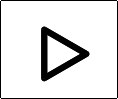
\includegraphics[width=3.0cm,trim=4 4 8 4,clip]{./images/disegnare/disegnare-34.png}
   \label{dis-34}
\end{figure}
\end{minipage} \hfill

\vskip 1cm

Possiamo alterare la rifinitura dei vertici facendo precedere il codice precedente dall'istruzione PENJOINT e un opportuno argomento. Le possibilità sono le seguenti:

\vskip 1cm

\begin{figure}[H]
   \centering
   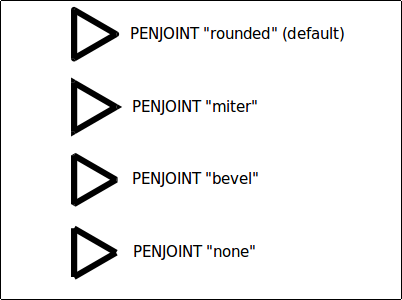
\includegraphics[width=10.0cm,trim=8 8 8 8,clip]{./images/disegnare/disegnare-35.png}
   \label{dis-35}
\end{figure}

\vskip 1cm

L'argomento  "rounded " significa arrotondato – (default) non va scritto nel comando: lo abbiamo aggiunto per dire che quello è il comportamento standard se non si specifica nulla. Se tuttavia si è appena utilizzata una delle altre opzioni, allora va usato esplicitamente il comando \textbf{PENJOINT  "rounded "}, per ottenere i vertici arrotondati. L'argomento  "miter " significa  "mitria " e sta peer  "giunto a mitria ", o  "giunto a quartabono ", che è quello che si realizza nelle cornici dei quadri tagliano i singoli regoli della cornice in maniera che i vertici risultino a punta.  "bevel " significa vertici smussati.

\subsubsection{PENCAP (forma delle estremità dei segmenti)}

Con questo comando si possono controllare gli estremi di un segmento:

\vskip 1cm

\begin{figure}[H]
   \centering
   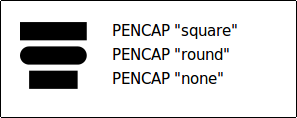
\includegraphics[width=10.0cm,trim=8 8 8 8,clip]{./images/disegnare/disegnare-36.png}
   \label{dis-36}
\end{figure}

\vskip 1cm

Per commentare il comportamento di questo comando, e anche per ricapitolare un po' la scrittura del codice in Logo, analizziamo il codice che è servito a produrre questa figura, omettendo, per semplicità, la parte che produce le scritte a destra. Per capire più facilmente, orientiamoci mediante i punti cardinali, così orientati:

\vskip 1cm

\begin{figure}[H]
   \centering
   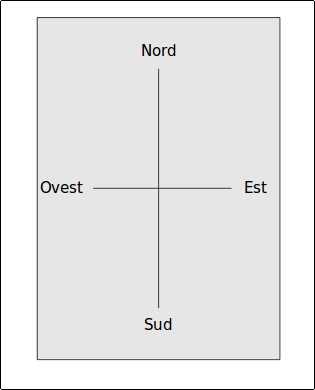
\includegraphics[width=10.0cm,trim=8 8 8 8,clip]{./images/disegnare/disegnare-37.png}
   \label{dis-37}
\end{figure}

\vskip 1cm

Vediamo quindi il codice seguente:

\pagebreak

\vskip 1cm

%https://en.wikibooks.org/wiki/LaTeX/Source_Code_Listings
\lstset{literate=
  {á}{{\'a}}1 {é}{{\'e}}1 {í}{{\'i}}1 {ó}{{\'o}}1 {ú}{{\'u}}1
  {Á}{{\'A}}1 {É}{{\'E}}1 {Í}{{\'I}}1 {Ó}{{\'O}}1 {Ú}{{\'U}}1
  {à}{{\`a}}1 {è}{{\`e}}1 {ì}{{\`i}}1 {ò}{{\`o}}1 {ù}{{\`u}}1
  {À}{{\`A}}1 {È}{{\'E}}1 {Ì}{{\`I}}1 {Ò}{{\`O}}1 {Ù}{{\`U}}1
  {ä}{{\"a}}1 {ë}{{\"e}}1 {ï}{{\"i}}1 {ö}{{\"o}}1 {ü}{{\"u}}1
  {Ä}{{\"A}}1 {Ë}{{\"E}}1 {Ï}{{\"I}}1 {Ö}{{\"O}}1 {Ü}{{\"U}}1
  {â}{{\^a}}1 {ê}{{\^e}}1 {î}{{\^i}}1 {ô}{{\^o}}1 {û}{{\^u}}1
  {Â}{{\^A}}1 {Ê}{{\^E}}1 {Î}{{\^I}}1 {Ô}{{\^O}}1 {Û}{{\^U}}1
  {œ}{{\oe}}1 {Œ}{{\OE}}1 {æ}{{\ae}}1 {Æ}{{\AE}}1 {ß}{{\ss}}1
  {ű}{{\H{u}}}1 {Ű}{{\H{U}}}1 {ő}{{\H{o}}}1 {Ő}{{\H{O}}}1
  {ç}{{\c c}}1 {Ç}{{\c C}}1 {ø}{{\o}}1 {å}{{\r a}}1 {Å}{{\r A}}1
  {€}{{\euro}}1 {£}{{\pounds}}1 {«}{{\guillemotleft}}1
  {»}{{\guillemotright}}1 {ñ}{{\~n}}1 {Ñ}{{\~N}}1 {¿}{{?`}}1
}
\lstset{extendedchars=true, basicstyle=\scriptsize} 
\begin{lstlisting}[frame=single]  % Start your code-block

CLEARSCREEN		; cancello il foglio (solo la parte grafica)
HOME			; partenza: tartaruga al centro che punta a Nord 
HIDETURTLE		; nascondo la tartaruga
PENWIDTH 15		; imposto lo spessore della linea a 15 pt

RIGHT 90		; ruoto 90\degree a destra così la tartaruga 
			; punta a Est in modo 
			; da tracciare da sinistra a destra
				
PENCAP  "square "		; imposto il modo  "estremità quadrate "
FORWARD 40		; disegno 40 pt di linea 
			; (Ovest -> Est)
PENUP  			; alzo la penna
RIGHT 90 FORWARD 20	; giro a destra di 90\degree (punto a Sud) e 
			; calo di 20 pt
LEFT 90 BACK 40		; rigiro a sinistra (punto a Est) e torno 
			; indietro  (Est -> Ovest) di 40 pt
PENDOWN			; abbasso la penna

PENCAP  "round "	; imposto il modo  "estremità arrotondate "
FORWARD 40		; disegno 40 pt di linea 
			; (Ovest -> Est)
PENUP			; alzo la penna
RIGHT 90 FORWARD 20	; giro a destra di 90\degree (punto a Sud) e 
			; calo di 20 pt
LEFT 90 BACK 40		; rigiro a sinistra (punto a Est), torno 
			; indietro ( Est -> Ovest) di 40 pt 
PENDOWN			; alzo la penna

PENCAP  "none "		; imposto il modo  "estremità arrotondate "
FORWARD 40		; disegno 40 pt di linea 
			; (Ovest -> Est)
PENUP			; alzo la penna

\end{lstlisting}

\vskip 1cm

Abbiamo evidenziato le istruzioni che realizzano i tre tratti, che riportiamo ancora qui:

\vskip 1cm

\begin{figure}[H]
   \centering
   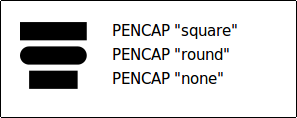
\includegraphics[width=10.0cm,trim=8 8 8 8,clip]{./images/disegnare/disegnare-36.png}
   \label{dis-38}
\end{figure}

\vskip 1cm

Ecco, si vede che in realtà sono stati disegnati tutti e tre con la stessa lunghezza di 40 pt e invece non sembra che siano venuti uguali. Questo per capire come funziona il comando PENCAP. Il tratto disegnato con assenza di specifiche per le estremità ( "effetto none ")  è lungo 40 pt. Quindi quelli con gli effetti  "round " e  "square " vengono più lunghi. Si capisce da qui che gli arrotondamenti sono aggiunti alla lunghezza normale e che l'effetto  "square " è ottenuto risquadrando gli arrotondamenti.

Va da sè che si tratta di un aspetto marginale. Abbiamo colto l'occasione per mettere in luce la notevole raffinatezza di LibreLogo, per abituarci ulteriormente a muoversi nel foglio e pensare graficamente. 

\subsubsection{PENSTYLE (tratteggio segmenti)}

Con questa istruzione si può determinare la continuità del tracciamento, per produrre linee tratteggiate di vario tipo:

\vskip 1cm

\begin{figure}[H]
   \centering
   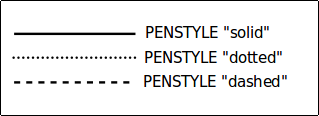
\includegraphics[width=10.0cm,trim=8 8 8 8,clip]{./images/disegnare/disegnare-38.png}
   \label{dis-39}
\end{figure}

\vskip 1cm

È anche possibile regolare in qualsiasi modo il tratteggio. Per esempio con l'istruzione \textbf{PENSTYLE [3, 1mm, 2, 4mm, 1mm]} si ottiene il tratteggio:

\vskip 1cm

\begin{figure}[H]
   \centering
   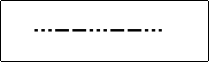
\includegraphics[width=10.0cm,trim=8 8 8 8,clip]{./images/disegnare/disegnare-39.png}
   \label{dis-40}
\end{figure}

\vskip 1cm

Queste sono le regole: 

\begin{itemize}
\item Parametro 1: numero di punti
\item Parametro 2: lunghezza dei punti
\item Parametro 3: numero di tratti
\item Parametro 4: lunghezza dei tratti
\item Parametro 5: lunghezza spazi
\item Parametro 6: opzionale, se vale 2 allora i rettangoli sono forzati a quadrati
\end{itemize}

\subsubsection{FILLSTYLE (tratteggio superfici)}

L'istruzione FILLSTYLE 1, precedente al disegno di una figura, causa il tratteggio della medesima. Il parametro numerico determina lo stile del tratteggio, nel modo seguente:


\vskip 1cm

\begin{figure}[H]
   \centering
   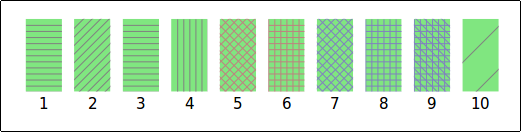
\includegraphics[width=10.0cm,trim=8 8 8 8,clip]{./images/disegnare/disegnare-40.png}
   \label{dis-41}
\end{figure}

\vskip 1cm

Anche qui, è possibile personalizzare lo schema del tratteggio, utilizzando dei parametri aggiuntivi:

\vskip 1cm

\begin{scriptsize}
\begin{minipage}{0.50\textwidth}
\begin{itemize}[itemsep=-3pt,parsep=2pt]
\item[] \textbf{FILLSTYLE [2,  "red ", 3pt, 15\degree]}           
\end{itemize}
\end{minipage}
\end{scriptsize}
\begin{minipage}{0.3\textwidth}
\begin{figure}[H]
   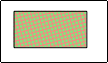
\includegraphics[width=3.0cm,trim=4 4 8 4,clip]{./images/disegnare/disegnare-41.png}
   \label{dis-42}
\end{figure}
\end{minipage} \hfill

\vskip 1cm

\subsection{Conclusioni}

Con queste istruzioni si conclude la parte della nostra esplorazione di LibreLogo dedicata al disegno. Abbiamo imparato i comandi fondamentali per muovere la tartaruga nello spazio del foglio, sia per disegnare che per muoversi semplicemente. Abbiamo imparato a muoversi come farebbe una tartaruga vera, o come facciamo noi in città, seguendo un percorso continuo, immaginando un “avanti” di fronte alla nostra posizione corrente, un indietro, una destra e una sinistra. Ma abbiamo anche visto come fare a muoversi con il “teletrasporto”, come se inserendo le coordinate nel navigatore satellitare l'automobile ci portasse istantaneamente in quel luogo, senza dover seguire tutto un percorso sulla superficie terrestre; o come si muove il cavallo negli scacchi, saltando direttamente a una casella distante 1+2 o 2+1 posizioni.   Abbiamo visto come si codificano i colori per decorare sia le linee che le superfici. Con tutto questo ci è sembrato di potere fare ormai disegnare tutto sul foglio, ma poi abbiamo subito scoperto delle istruzioni per disegnare direttamente le principali figure geometriche: quadrati, rettangoli, cerchi e ellissi, con alcune varianti, come settori, segmenti e archi di ellissi (o cerchi), oppure rettangoli con i vertici arrotondanti. Quindi abbiamo introdotto il primo degli elementi fondamentali che caratterizzano un vero e proprio linguaggio di programmazione: il concetto di variabile, con il quale possiamo usare dei simboli letterari generici per designare specifiche quantità – distanze, angoli e altro – senza doversi preoccupare di assegnare loro precisi valori numerici; una caratteristica fondamentale che che conferisce al linguaggio una potenzialità simile a quella che sta alla base dell'algebra, con il calcolo simbolico. Non abbiamo esplorato tutta la potenzialità che soggiace al concetto di variabile, ma solo evidenziato quanto ci bastava per illustrare i movimenti nel foglio basati sull'impiego delle coordinate spaziali. Per fare questo abbiamo dovuto considerare un particolare tipo di variabile che è il vettore, composto a sua volta da più numeri – due se si tratta di un “vettore posizione” su di una superficie. Infine abbiamo visto che si possono usare altri comandi ancora per determinare i particolari grafici sia del tratto (colore, spessore, estremità, giunzioni) che delle superfici (colore, tratteggi). A questo punto, nuovamente, ci può parere di avere a disposizione di uno strumento potente per produrre grafica da inserire nei documenti. E effettivamente si possono fare senza dubbio tantissime cose con i comandi che abbiamo visto fino ad ora. In realtà, dal punto di vista del linguaggio di programmazione, abbiamo solo visto una piccola parte delle sue potenzialità. Si tratta di costrutti che stanno alla base di tutti i linguaggi di programmazione e che conferiscono le straordinarie capacità di flessibilità e generalizzazione agli innumerevoli tipi di software che tutti conosciamo ma soprattutto usiamo inconsapevolmente in ormai qualsiasi congegno.



















